\documentclass[11pt,a4paper]{article}
\usepackage[utf8]{inputenc}
\usepackage[T1]{fontenc}
\usepackage{lmodern}
\usepackage[italian]{babel}
\usepackage{geometry}
\usepackage{url}
\usepackage{hyperref}
\usepackage{parskip}
\usepackage{csquotes}
\usepackage{graphicx}
\usepackage{pdfpages}
\usepackage[backend=biber,style=authoryear,sorting=ynt]{biblatex}

\addbibresource{pubblicazioni.bib}

\geometry{margin=2.5cm}

\hypersetup{
    colorlinks=true,
    linkcolor=black,
    urlcolor=blue,
    citecolor=black
}

\begin{document}

% Include the autocertificazione PDF
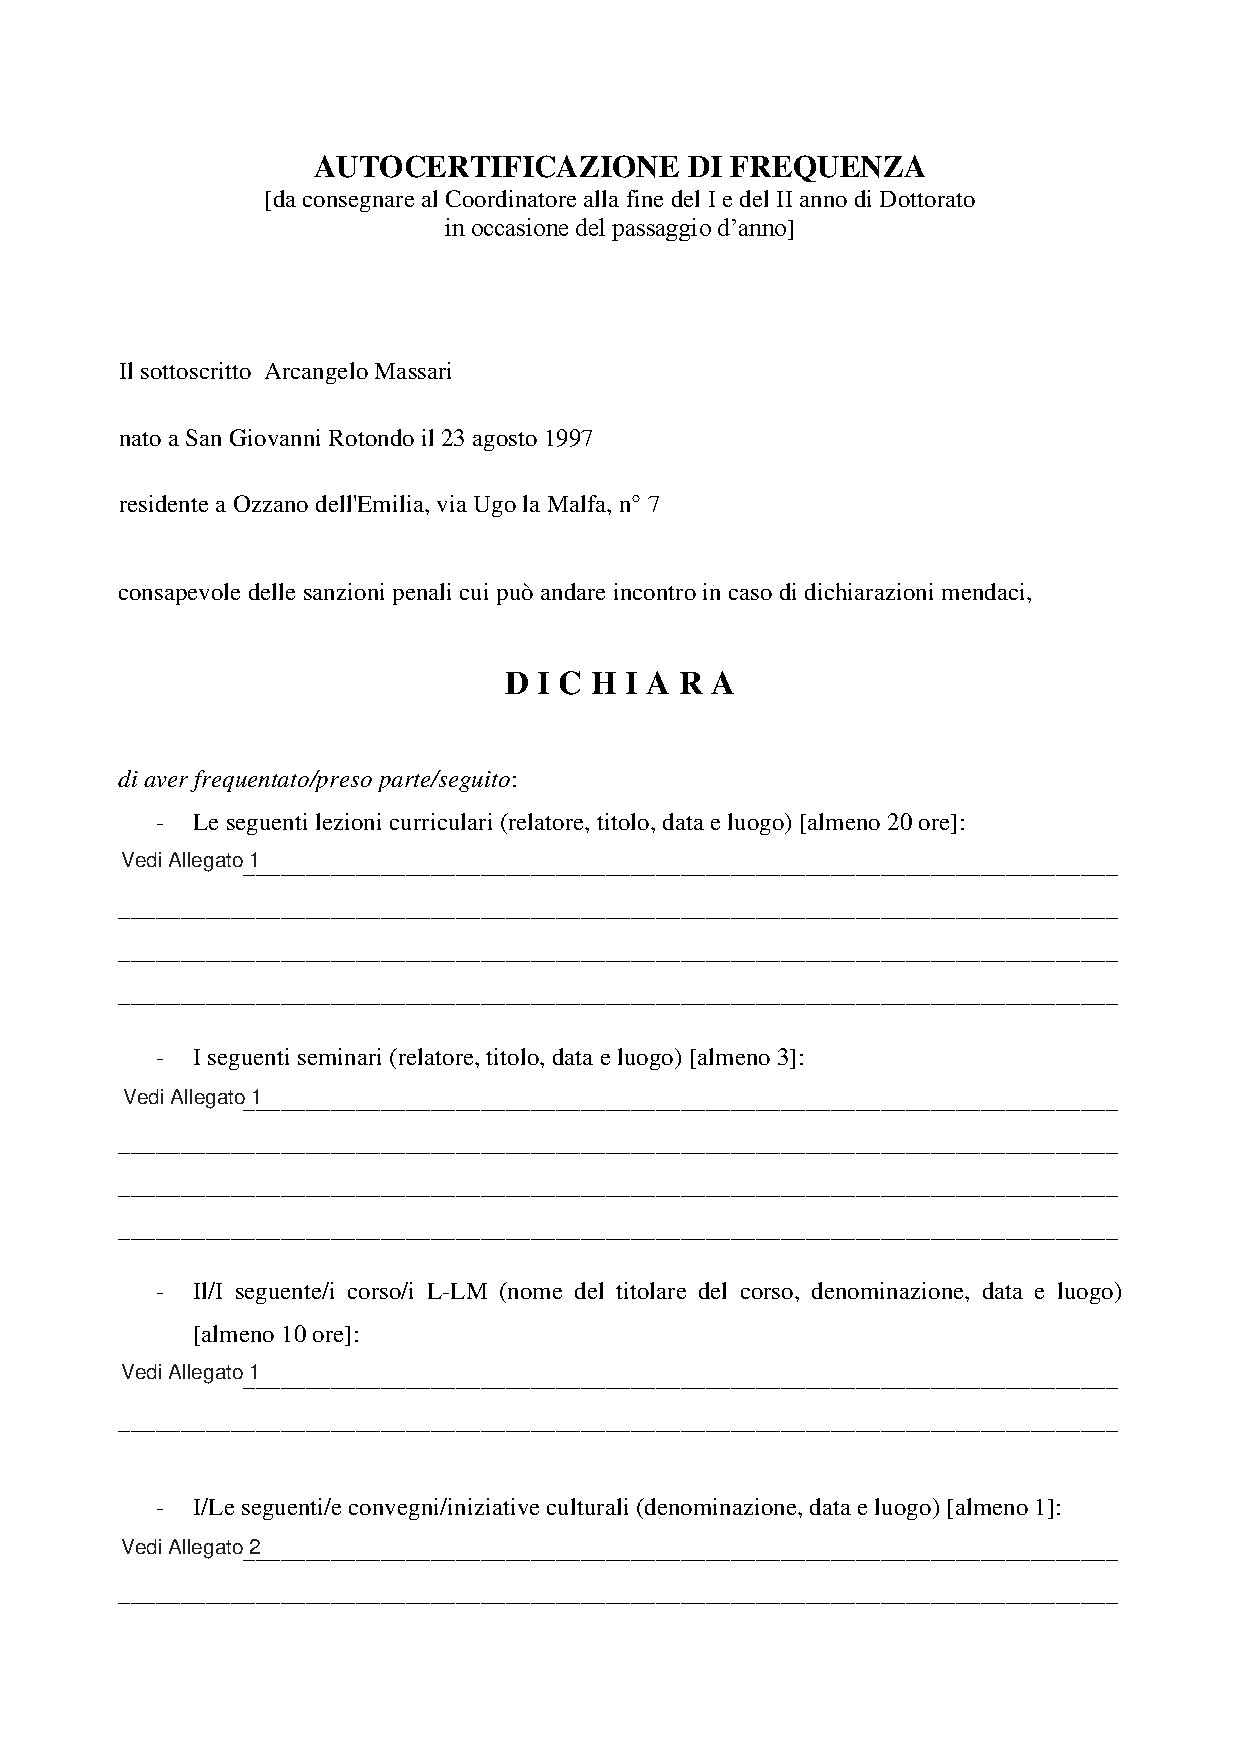
\includepdf[pages=-]{autocertificazione.pdf}

% ALLEGATO 1 - ATTIVITÀ FORMATIVE
\newpage
\begin{center}
{\Large \textbf{Allegato 1 -- Attività formative e didattiche}}\\[0.5cm]
{\large Arcangelo Massari}\\
{\large III anno di dottorato in Cultural Heritage in the Digital Ecosystem}
\end{center}

\section*{Nota sulla classificazione delle attività}

Le attività formative sono state organizzate secondo la classificazione aggiornata del programma dottorale, che prevede le seguenti categorie:
\begin{itemize}
    \item \textbf{Formazione disciplinare e multidisciplinare}: comprende le lezioni curriculari e i seminari disciplinari
    \item \textbf{Formazione relativa alle competenze trasversali}: include corsi trasversali e competenze complementari
    \item \textbf{Formazione extracurriculare}: attività formative aggiuntive
\end{itemize}

Questa classificazione rispecchia e soddisfa i requisiti dell'autocertificazione di frequenza, distribuendo le attività richieste (lezioni curriculari, seminari, corsi L-LM) nelle categorie sopra indicate.

\setcounter{section}{0}
\section{Formazione disciplinare e multidisciplinare}

LUDI Seminar Series: ``L'importanza di fare una buona impressione: vicende e progetti editoriali della Typographia Medicea delle lingue orientali (Roma, 1584-1614)'' di Sara Fani (AMS Università di Bologna). Frequentato online, 10 ottobre 2024, 14:00-17:00.

LUDI Seminar Series: ``La biblioteconomia nel contesto internazionale. Esperienze e progetti'' di Rossana Morriello (Università di Firenze). Frequentato online, 15 novembre 2024, 10:00-12:00.

``Revealing Connections: Leveraging Linked Open Data to discover knowledge through ResearchSpace''. Seminario di una giornata su archivi semantici digitali e tecnologie Linked Open Data. Aula Giorgio Prodi, Piazza San Giovanni in Monte, 2, Bologna, 28 novembre 2024, 9:30-17:00.

``Tweets or posts on X as sources of information'' di Elisavet Chantavaridou (Università di West Attica). Frequentato online, 10 dicembre 2024, 9:00-11:00.

``nodegoat: database for historical research and the Digital Humanities'' di Pim van Bree e Geert Kessels (Lab1100). Frequentato online, 6 marzo 2025, 10:00-12:00.

``Workshop PRIN Atlas'' della Prof.ssa Marilena Daquino. Aula Affreschi, Via Zamboni 34, Bologna, 26 marzo 2025, 10:00-17:00.

``AI Literacies in the Digital Humanities: Ethics, Archives, and Critical Thinking'' di Moisés Rockembach. Frequentato online, 17 giugno 2025, 10:00-13:00.

``Biblioteche digitali e IIIF. Caratteristiche, innovazioni e applicazioni'' di Fabio Cusimano. Presentazione del libro. Frequentato online, 4 luglio 2025, 15:00-17:00.

\section{Formazione relativa alle competenze trasversali}

``Frontiere dell'intelligenza artificiale'' di Giovanni Colavizza, 20 giugno 2025, 14:00-17:00.

``Artificial Intelligence Tools for Content Production in Academia'' di Paolo Torroni e Alessandro Gallo. Bologna, 26 maggio 2025, 23 giugno 2025, 30 giugno 2025, 15:00-18:00.

``Nuove macchine e antichi saperi: IA, Supercalcolo e dati per il patrimonio culturale''. Convegno su intelligenza artificiale, supercalcolo e dati per il patrimonio culturale. Frequentato online, 3 dicembre 2024, 9:00-13:00.

``Using Generative Artificial Intelligence for processing tweets'' di Elisavet Chantavaridou (Università di West Attica). Frequentato online, 6 dicembre 2024, 15:00-16:30.

\section{Formazione extracurriculare}

Seminari Una-Her-Doc su teorie del patrimonio, metodologie e approcci partecipativi. Frequentato online, 12 novembre 2024.

Avvio del programma Una-Her-Doc per la nuova coorte e seminari sulle teorie fondamentali. Frequentato online, 22 gennaio - 22 febbraio 2025.

Una-Her-Doc - Seminari sulle teorie fondamentali. Frequentato online, 7 marzo 2025.

Seminari Una-Her-Doc su teorie fondamentali e metodologia. Frequentato online, 19-20 giugno 2025.


% ALLEGATO 2 - CONVEGNI E INIZIATIVE CULTURALI
\newpage
\begin{center}
{\Large \textbf{Allegato 2 -- Convegni e iniziative culturali}}\\[0.5cm]
{\large Arcangelo Massari}\\
{\large III anno di dottorato in Cultural Heritage in the Digital Ecosystem}
\end{center}

\setcounter{section}{0}
\section{Disseminazione}

\textbf{PhD Workshop UnaEuropa}: ``Museums and New Challenges: virtual technologies, social responsibility and environmental sustainability''\\
\textit{Luogo}: Bologna, Italia\\
\textit{Data}: 5-10 maggio 2025\\
\textit{Descrizione}: Workshop internazionale per dottorandi nell'ambito del patrimonio culturale, focalizzato sulle nuove sfide che i musei devono affrontare in termini di tecnologie virtuali, responsabilità sociale e sostenibilità ambientale.\\
\textit{Presentazione}: ``HERITRACE: A User-Friendly Semantic Data Editor with Change Tracking and Provenance Management for Cultural Heritage Institutions''. Presentazione di HERITRACE, uno strumento web-based progettato per colmare il divario tra tecnologie semantiche complesse e l'expertise degli operatori del patrimonio culturale. Il sistema presenta un'interfaccia user-friendly per la gestione di dati RDF, gestione completa della provenienza, change-tracking con funzionalità snapshot e personalizzazione flessibile attraverso linguaggi standard come SHACL e YAML.\\
\textit{DOI}: \url{https://doi.org/10.5281/zenodo.15375769}

\vspace{0.5cm}

\textbf{csv,conf,v9}\\
\textit{Luogo}: Bologna, Italia\\
\textit{Data}: 10-11 settembre 2025\\
\textit{Descrizione}: Conferenza internazionale dedicata alla gestione e analisi di dati strutturati.\\
\textit{Presentazione}: ``Mapping the unmapped citation landscape: how crowdsourcing will fill the citation gap''. La presentazione esamina il problema dell'invisibilità delle citazioni nell'editoria accademica, particolarmente per le riviste del Sud Globale. Basandosi su ricerche esistenti che mostrano come tra oltre 52.000 riviste Open Journal Systems (OJS) mondiali, il 79,9\% si trova nel Sud Globale, con il 98,8\% invisibile a Web of Science e il 94,3\% invisibile a Scopus, la presentazione introduce una soluzione collaborativa sviluppata attraverso una partnership tra OpenCitations, Public Knowledge Project (PKP) e Leibniz Information Centre. La soluzione implementa un flusso di lavoro integrato in OJS che consente l'invio automatico di metadati bibliografici e citazioni a OpenCitations.\\
\textit{DOI}: \url{https://doi.org/10.5281/zenodo.17098599}

% ALLEGATO 3 - PUBBLICAZIONI
\newpage
\begin{center}
{\Large \textbf{Allegato 3 -- Pubblicazioni e produzione scientifica}}\\[0.5cm]
{\large Arcangelo Massari}\\
{\large III anno di dottorato in Cultural Heritage in the Digital Ecosystem}
\end{center}

\section{Articoli su rivista}

\fullcite{massariHERITRACEUserFriendlySemantic2025}

\fullcite{massariRepresentingProvenanceTrack2025}

\fullcite{barzaghiProposalFAIRManagement2024}

\fullcite{sebastianReproducibleWorkflowCreation2025}

\section{Software rilasciati}

\fullcite{arcangelomassariOpencitationsHeritraceV2332025}

\fullcite{arcangelomassariOpencitationsTimeagnosticlibrary5042025}

\fullcite{arcangelomassariOpencitationsOc_metaV2132025}

\section{Presentazioni}

\fullcite{massariMappingUnmappedCitation2025}

\fullcite{massariPresentationHERITRACEUserFriendly2025}


\end{document}